%===================================== CHAP 5 =================================

\chapter{Results} \label{chap:results}

This chapter presents the results of the thesis work relevant for answering the research questions defined in \autoref{sec:research-questions}, for both the visualization tool and the case study. We will explain the process of generating the results and elaborate on their quality and reliability, but will save the discussion of their implications for \autoref{chap:discussion}.

\section{Visualization Tool} \label{sec:visualization-tool-results}

This section will focus on showcasing a representative selection of visualizations generated using the various visualization techniques implemented in the visualization tool. The visualizations were produced using the tool, but we will display them as independent images instead of incorporated into the web interface. We refer the reader to \autoref{app:user-manual} and \autoref{app:callbacks-api} for an overview of the implemented visualization tool.

\subsection{Example Networks} \label{sec:example-networks}

The visualization results were produced using two different example \acrshortpl{ann}. The first network is a simple \acrshort{cnn} trained on the \acrfull{mnist} dataset\footnote{http://yann.lecun.com/exdb/mnist/}, which is commonly used as a toy problem. This network is quickly trained from scratch to near perfect accuracy, which allowed us to easily show how the visualizations evolve throughout the training progress. The second network is the more advanced \acrshort{vgg} network, more specifically the 16-layer version in configuration D \cite{vgg}. In this case, we used a model with weights pretrained on \acrshort{ilsvrc} 2012 image set \cite{imagenet}. Some of the visualizations, such as those from the deconvolutional network technique, require a large network with many convolutional layers to demonstrate their full capabilities. Using a fully trained \acrshort{vgg} model, we were able to present a second set of visualizations illustrating more complex features, without having to spend a large amount of time training the network. The \acrshort{vgg} network also allowed us to display how the visualizations handle RGB images, compared to the grayscale images of the \acrshort{mnist} dataset. Both networks were implemented following examples provided by Keras, and in the following sections we describe their implementations and training processes in detail.\\

\noindent Note that there are several ways to count the number of layers in an \acrshort{ann}. Some conventions do not include pooling or flattening layers, or even the input and output layers. To ensure consistency when describing the network architectures, we will define the number of layers as the number of Keras layers, as listed in their documentation \cite{keras-documentation}.

\subsubsection{The \acrshort{mnist} Network}

The \acrshort{mnist} network is a simple \acrshort{cnn} with three convolutional layers, including the max pooling layer. It is trained on the \acrshort{mnist} dataset, which contains 60,000 28x28 grayscale images of handwritten digits. The network architecture can be seen in \autoref{fig:mnist-architecture}, and was created following an example implementation from Keras \footnote{https://github.com/fchollet/keras/blob/master/examples/mnist\_cnn.py}. The network consists of 10 layers, where three are convolutional and pooling layers, and two are fully connected, denoted as dense layers in Keras. In addition to an input layer, there are also two dropout layers to prevent overfitting, and a flattening layer to convert the 3D output from the convolutional part to 1D input for the fully connected part. The model is trained using an AdaDelta optimizer with default Keras values\footnote{https://keras.io/optimizers/\#adadelta} to minimize the categorical cross-entropy loss. \\

\noindent To generate the results, the network was trained for two epochs with a batch size of 128, shuffling the data at each epoch. In addition to the 60,000 training images, 10,000 images were used as validation data. The 10 images in \autoref{fig:mnist-input-images} were extracted from the validation dataset to be used as visualization input images. The training process was repeated using each of these images as input for the visualizations. The visualizations were produced five times during each epoch, in addition to once at the very beginning of the training, giving a total of 11 different sets of visualization results for each of the 10 digits. The produced visualizations were manually processed and a representative selection were extracted, presented in \autoref{sec:mnist-vis-results}.

\begin{figure}
\begin{center}
\begin{tabular}{ccccc}
\subfloat['0': 100\%]{
\includegraphics[width = 0.61in]{fig/results/input_mnist/test0.png}} & 
\subfloat['1': 100\%]{
\includegraphics[width = 0.61in]{fig/results/input_mnist/test1.png}} & 
\subfloat['2': 100\%]{
\includegraphics[width = 0.61in]{fig/results/input_mnist/test2.png}} &
\subfloat['3': 100\%]{
\includegraphics[width = 0.61in]{fig/results/input_mnist/test3.png}} & 
\subfloat['4': 100\%]{
\includegraphics[width = 0.61in]{fig/results/input_mnist/test4.png}} \\
\subfloat['2': 100\%]{
\includegraphics[width = 0.61in]{fig/results/input_mnist/test5.png}} &
\subfloat['6': 100\%]{
\includegraphics[width = 0.61in]{fig/results/input_mnist/test6.png}} & 
\subfloat['7': 100\%]{
\includegraphics[width = 0.61in]{fig/results/input_mnist/test7.png}} & 
\subfloat['8': 100\%]{
\includegraphics[width = 0.61in]{fig/results/input_mnist/test8.png}} &
\subfloat['9': 100\%]{
\includegraphics[width = 0.61in]{fig/results/input_mnist/test9.png}} \\
\end{tabular}
\caption[Visualization input images for \acrshort{mnist}]{The images used as visualization input for the \acrshort{mnist} network, captioned with their corresponding classification result and confidence at stage 1 of training. Note that \textbf{f} was incorrectly classified as '2'. At stage 2, all images were correctly classified with 100\% certainty.}
\label{fig:mnist-input-images}
\end{center}
\end{figure}

\subsubsection{The \acrshort{vgg} Network}

The \acrshort{vgg} network is a significantly deeper \acrshort{cnn} than the first network. It consists of five blocks of 3-4 convolutional layers each, including the max pooling layers, followed by a flattening layer and three fully connected layers, for a total of 23 layers. The full architecture can be seen in \autoref{fig:vgg-architecture}. The \acrshort{vgg} model used has weights trained on the \acrshort{ilsvrc} image set and is available through the Keras Applications module\footnote{https://keras.io/applications/\#vgg16}\footnote{https://github.com/fchollet/keras/blob/master/keras/applications/vgg16.py}. \\

\noindent As mentioned, the \acrshort{vgg} network employed is a fully trained model, meaning that the results generated using this network only consist of visualizations produced at the very end of the training process. The three visualization input images seen in \autoref{fig:vgg-input-images} were used to produce visualizations, with the image in \autoref{fig:vgg-input-image1} being the main visualization input image. The other two images were used to produce visualizations to compare to. They were selected as they are both related to the main image in some way. Specifically, one contains a bicycle similar to the tricycle in the main image, and the other contains a woman with similar features to the girl in the main image. The visualization techniques were repeated a number of times with various configurations and the different input images. The resulting visualizations were manually processed, and a representative selection are presented in \autoref{sec:vgg-vis-results}.

\begin{figure}[p]
\begin{center}
\begin{tabular}{c}
\subfloat['tricycle, trike, velocipede': 99.95\%]{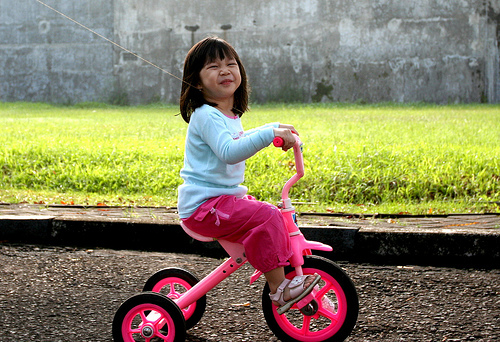
\includegraphics[width=0.5\textwidth]{fig/results/input_vgg/girlonbike.JPEG}\label{fig:vgg-input-image1}} \\
\subfloat['cliff, drop, drop-off': 64.35\%]{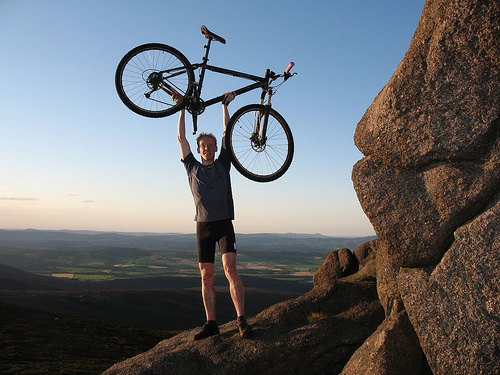
\includegraphics[width=0.5\textwidth]{fig/results/input_vgg/biking.JPEG}} \\
\subfloat['sombrero': 50.91\%]{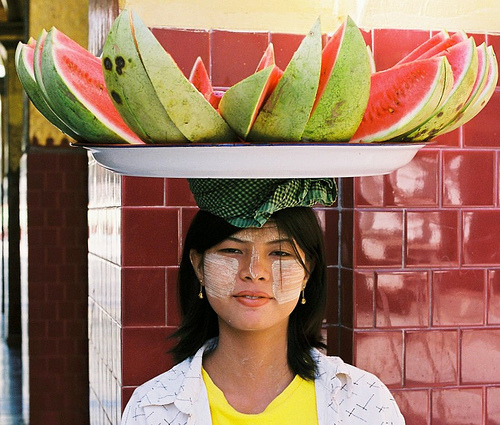
\includegraphics[width=0.5\textwidth]{fig/results/input_vgg/girl.JPEG}} \\
\end{tabular}
\caption[Visualization input images for \acrshort{vgg}]{The images used as visualization input for the \acrshort{vgg} network, captioned with their corresponding classification result and confidence.}
\label{fig:vgg-input-images}
\end{center}
\end{figure}

\begin{figure}
    \begin{minipage}{0.5\textwidth}
        \centering
            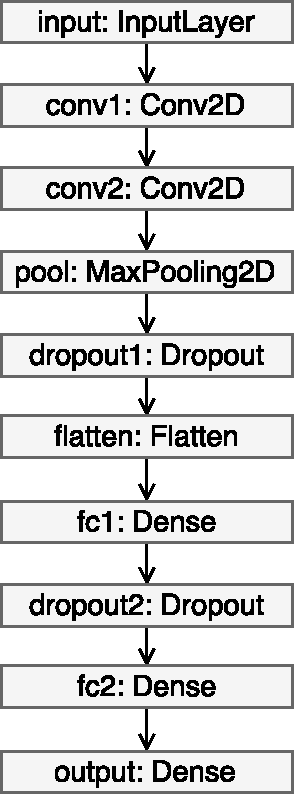
\includegraphics[width=0.6\textwidth]{fig/mnist_keras.pdf}
            \caption{Architecture of the \acrshort{mnist} network with layer names and types. Note that the layer type refers to the Keras 2 \acrshort{api}.}
            \label{fig:mnist-architecture}
    \end{minipage}
    \begin{minipage}{0.4\textwidth}
        \centering
            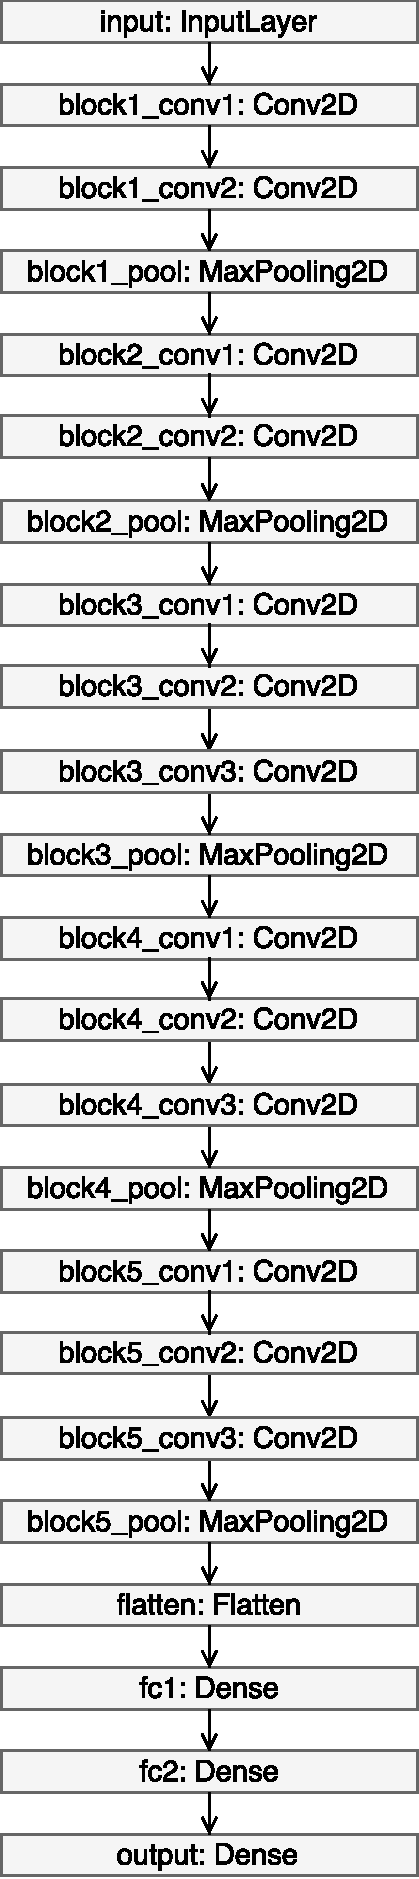
\includegraphics[width=0.7\textwidth]{fig/vgg_keras.pdf}
            \caption{Architecture of the \acrshort{vgg} network with layer names and types. Note that the layers refer to the Keras 2 \acrshort{api}.}
            \label{fig:vgg-architecture}
    \end{minipage}
\end{figure}

\subsection{\acrshort{mnist} Visualization Results} \label{sec:mnist-vis-results}

This section presents the visualization results produced by the various visualization techniques for the \acrshort{mnist} network.

\subsubsection{Training Progress}

The visualizations of the training progress can be seen in \autoref{fig:mnist-training-progress}, showing the batch accuracy and batch loss. To produce these visualizations, the training was expanded from two epochs to six, to show a longer graph. The blue lines display the training accuracy and loss, while the green dots display the validation accuracy and loss at each epoch.

% noe om at det ikke er variasjon i training progress?

\begin{figure}[p]
\begin{center}
\begin{tabular}{c}
\subfloat{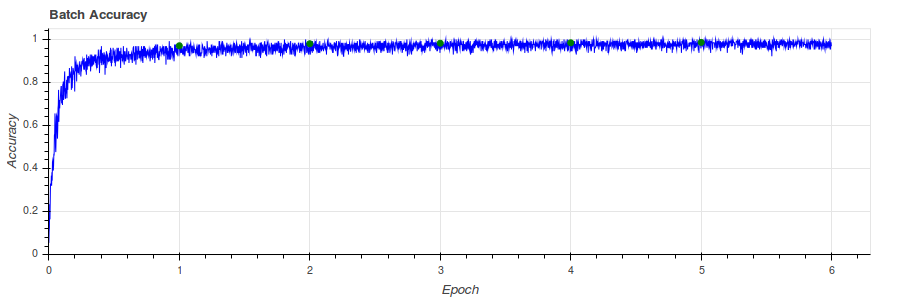
\includegraphics[width=1\textwidth]{fig/results/training_progress/accuracy.png}} \\
\subfloat{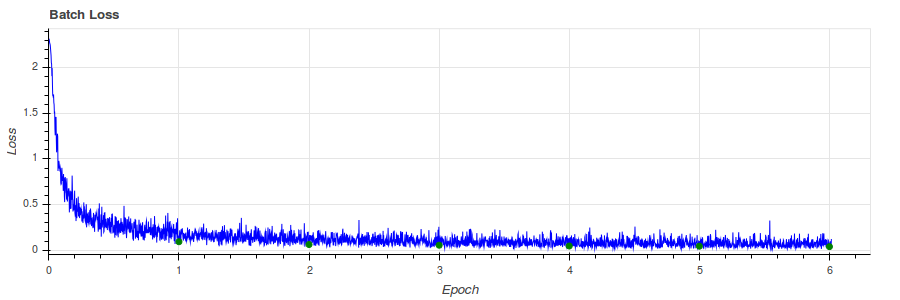
\includegraphics[width=1\textwidth]{fig/results/training_progress/loss.png}} \\
\end{tabular}
\caption[Batch accuracy and loss for \acrshort{mnist} network]{Batch accuracy and loss over epoch for the \acrshort{mnist} network. Validation accuracy and loss displayed as green dots at each epoch. Note that the validation accuracy and loss are best viewed electronically.}
\label{fig:mnist-training-progress}
\end{center}
\end{figure}

\subsubsection{Layer Activations}

\autoref{fig:mnist-layer-act-all} shows the fully trained network's layer activations for all layers, except the flattening and dropout layers. Flattening layers are excluded because they do not provide any extra information, and are generally too large to be presented in a readable manner. Dropout layers are excluded since they are identical to the preceding layer. The feature maps of the convolutional layers are displayed in a grid so that they can be viewed together all at once. The fully connected layers are displayed as pixels laid out horizontally, scaled to fit the width of the page. \\

\begin{figure}[p]
\captionsetup[subfigure]{labelformat=empty}
\begin{center}
\begin{tabular}{c}
\begingroup
\captionsetup[subfigure]{width=1in}
\subfloat[input]{\makebox[1in][c]{
\includegraphics[width = 0.4in]{fig/results/input_mnist/test0.png}}}\endgroup \\
\subfloat[conv1]{\frame{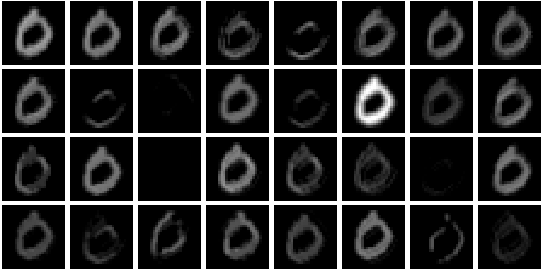
\includegraphics[width=0.6\textwidth]{fig/results/layeract_mnist/all_layers/layer_act_mnist_0_10_conv2d_1.png}}} \\
\subfloat[conv2]{\frame{\includegraphics[width=0.6\textwidth]{fig/results/layeract_mnist/all_layers/layer_act_mnist_0_10_conv2d_2.png}}} \\
\subfloat[pool]{\frame{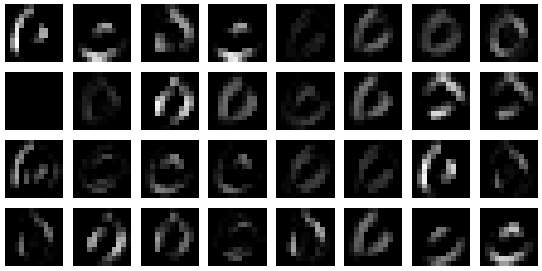
\includegraphics[width=0.5\textwidth]{fig/results/layeract_mnist/all_layers/layer_act_mnist_0_10_max_pooling2d_1.png}}} \\
\subfloat[fc1]{\frame{
\includegraphics[width=\textwidth]{fig/results/layeract_mnist/all_layers/layer_act_mnist_0_10_dense_1.png}}} \\
\subfloat[fc2]{\frame{
\includegraphics[width=\textwidth]{fig/results/layeract_mnist/all_layers/layer_act_mnist_0_10_dense_2.png}}} \\
\subfloat[output]{\frame{
\includegraphics[width=0.3\textwidth]{fig/results/layeract_mnist/all_layers/layer_act_mnist_0_10_dense_3.png}}} \\
\end{tabular}
\caption[Layer activations for all \acrshort{mnist} layers]{Layer activations for all layers of the \acrshort{mnist} network, excluding flattening and dropout layers, for visualization input image 0 after two epochs.}
\label{fig:mnist-layer-act-all}
\end{center}
\end{figure}

\noindent \autoref{fig:mnist-layer-act-conv2} illustrates the transition of the layer activations throughout the training process. It is illustrated by the \texttt{conv2} layer activations, as they show a progression that is easy to understand and interpret. The activations are shown at three stages: the first stage at the beginning of training, a middle stage halfway in the training, and a final stage at the end of training.

\begin{figure}[p]
\captionsetup[subfigure]{labelformat=empty}
\begin{center}
\begin{tabular}{c}
\subfloat[Stage 1]{\frame{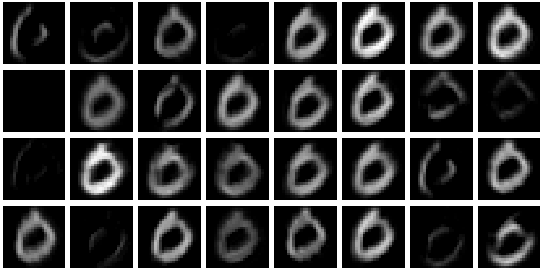
\includegraphics[width=0.8\textwidth]{fig/results/layeract_mnist/layer_act_mnist_0_1_conv2d_2.png}}} \\
\subfloat[Stage 5]{\frame{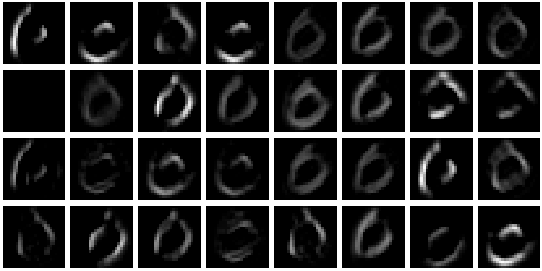
\includegraphics[width=0.8\textwidth]{fig/results/layeract_mnist/layer_act_mnist_0_5_conv2d_2.png}}} \\
\subfloat[Stage 10]{\frame{\includegraphics[width=0.8\textwidth]{fig/results/layeract_mnist/layer_act_mnist_0_10_conv2d_2.png}}} \\
\end{tabular}
\caption[Change in activations in \texttt{conv2} of \acrshort{mnist}]{Layer activations for the \texttt{conv2} layer of the \acrshort{mnist} network at various stages in the training process.}
\label{fig:mnist-layer-act-conv2}
\end{center}
\end{figure}

\subsubsection{Saliency Maps}

\autoref{fig:mnist-saliency} shows saliency maps at various stages of the training process for each of the visualization input images classified in \autoref{fig:mnist-input-images}. Note that stage 0 is an initial stage before the training has started. The illustration includes more of the earlier stages than later stages because most of the changes to the saliency map occur at the beginning of the training process.

\begin{figure}
\begin{center}
\begin{tabular}{ccccccc}
\textbf{Input} & \textbf{0} & \textbf{1} & \textbf{2} & \textbf{4} & \textbf{7} & \textbf{10} \\
\subfloat{
\includegraphics[width = 0.5in]{fig/results/input_mnist/test0.png}} &
\subfloat{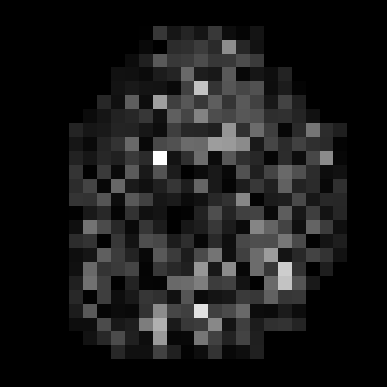
\includegraphics[width = 0.49in]{fig/results/saliency_mnist/saliency_mnist_0_0.png}} &
\subfloat{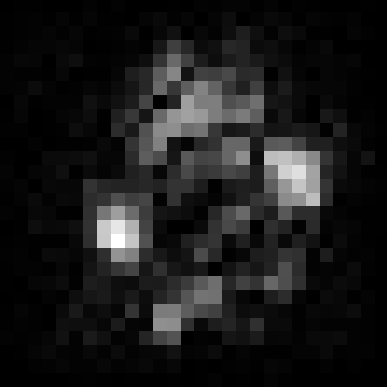
\includegraphics[width = 0.49in]{fig/results/saliency_mnist/saliency_mnist_0_1.png}} &
\subfloat{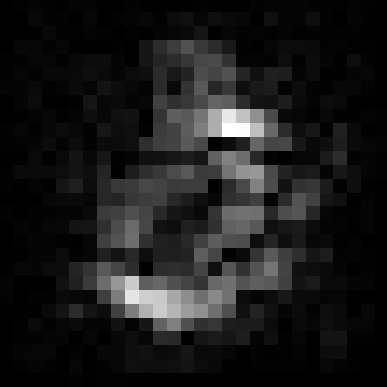
\includegraphics[width = 0.49in]{fig/results/saliency_mnist/saliency_mnist_0_2.png}} &
\subfloat{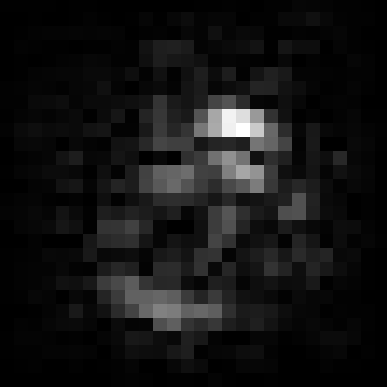
\includegraphics[width = 0.49in]{fig/results/saliency_mnist/saliency_mnist_0_4.png}} &
\subfloat{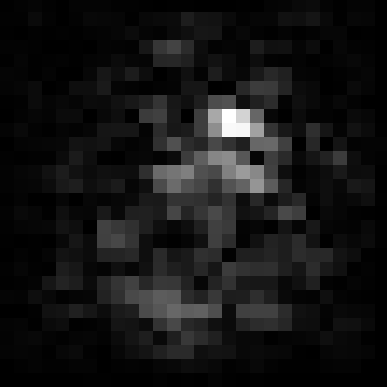
\includegraphics[width = 0.49in]{fig/results/saliency_mnist/saliency_mnist_0_7.png}} &
\subfloat{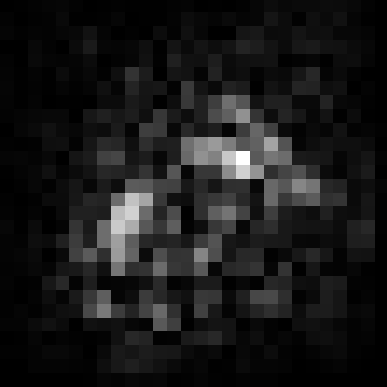
\includegraphics[width = 0.49in]{fig/results/saliency_mnist/saliency_mnist_0_10.png}} \\
\subfloat{
\includegraphics[width = 0.49in]{fig/results/input_mnist/test1.png}} & 
\subfloat{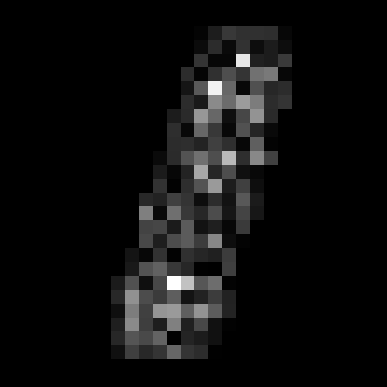
\includegraphics[width = 0.49in]{fig/results/saliency_mnist/saliency_mnist_1_0.png}} &
\subfloat{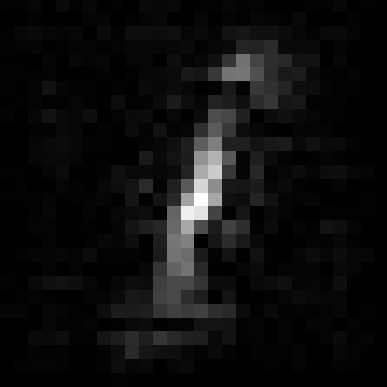
\includegraphics[width = 0.49in]{fig/results/saliency_mnist/saliency_mnist_1_1.png}} &
\subfloat{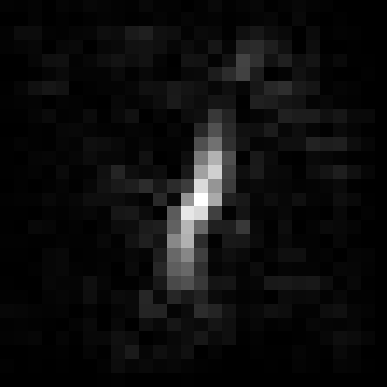
\includegraphics[width = 0.49in]{fig/results/saliency_mnist/saliency_mnist_1_2.png}} &
\subfloat{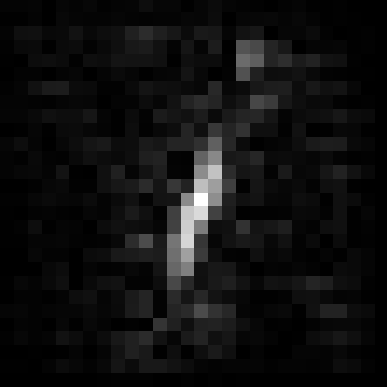
\includegraphics[width = 0.49in]{fig/results/saliency_mnist/saliency_mnist_1_4.png}} &
\subfloat{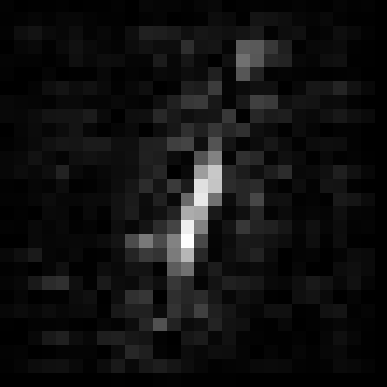
\includegraphics[width = 0.49in]{fig/results/saliency_mnist/saliency_mnist_1_7.png}} &
\subfloat{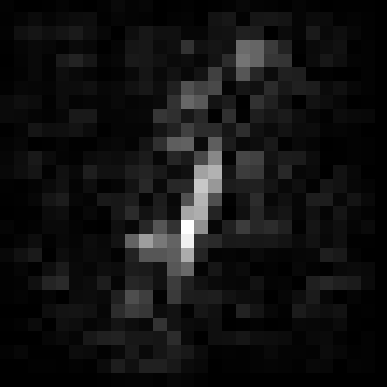
\includegraphics[width = 0.49in]{fig/results/saliency_mnist/saliency_mnist_1_10.png}} \\
\subfloat{
\includegraphics[width = 0.49in]{fig/results/input_mnist/test2.png}} &
\subfloat{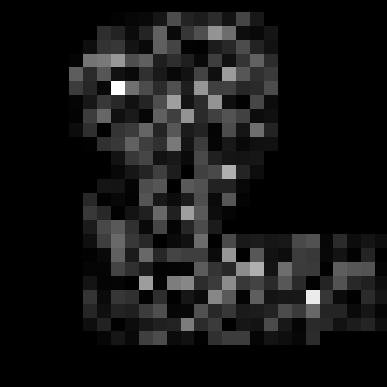
\includegraphics[width = 0.49in]{fig/results/saliency_mnist/saliency_mnist_2_0.png}} &
\subfloat{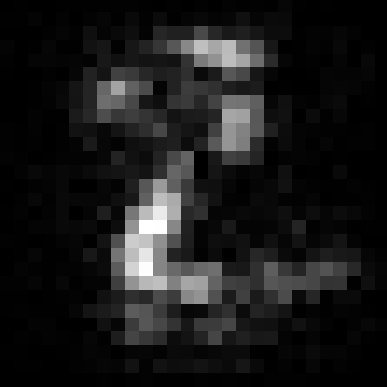
\includegraphics[width = 0.49in]{fig/results/saliency_mnist/saliency_mnist_2_1.png}} &
\subfloat{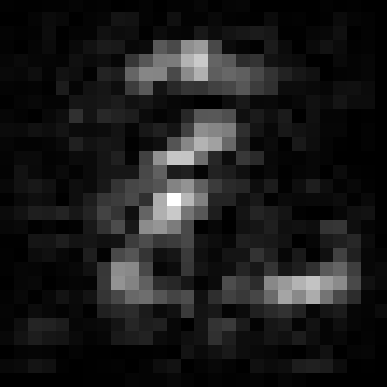
\includegraphics[width = 0.49in]{fig/results/saliency_mnist/saliency_mnist_2_2.png}} &
\subfloat{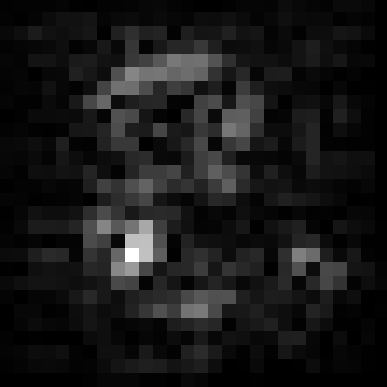
\includegraphics[width = 0.49in]{fig/results/saliency_mnist/saliency_mnist_2_4.png}} &
\subfloat{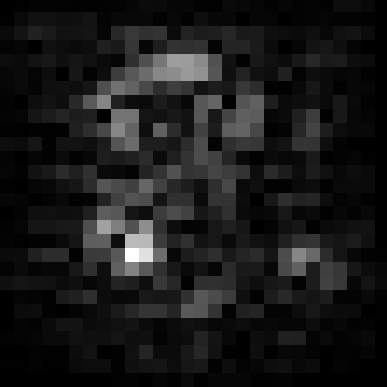
\includegraphics[width = 0.49in]{fig/results/saliency_mnist/saliency_mnist_2_7.png}} &
\subfloat{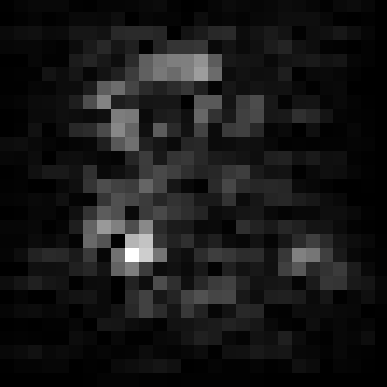
\includegraphics[width = 0.49in]{fig/results/saliency_mnist/saliency_mnist_2_10.png}} \\   
\subfloat{
\includegraphics[width = 0.49in]{fig/results/input_mnist/test3.png}} &
\subfloat{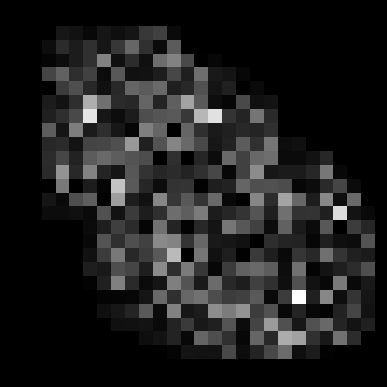
\includegraphics[width = 0.49in]{fig/results/saliency_mnist/saliency_mnist_3_0.png}} &
\subfloat{\includegraphics[width = 0.49in]{fig/results/saliency_mnist/saliency_mnist_3_1.png}} &
\subfloat{\includegraphics[width = 0.49in]{fig/results/saliency_mnist/saliency_mnist_3_2.png}} &
\subfloat{\includegraphics[width = 0.49in]{fig/results/saliency_mnist/saliency_mnist_3_4.png}} &
\subfloat{\includegraphics[width = 0.49in]{fig/results/saliency_mnist/saliency_mnist_3_7.png}} &
\subfloat{\includegraphics[width = 0.49in]{fig/results/saliency_mnist/saliency_mnist_3_10.png}} \\
\subfloat{\includegraphics[width = 0.49in]{fig/results/input_mnist/test4.png}} &
\subfloat{\includegraphics[width = 0.49in]{fig/results/saliency_mnist/saliency_mnist_4_0.png}} &
\subfloat{\includegraphics[width = 0.49in]{fig/results/saliency_mnist/saliency_mnist_4_1.png}} &
\subfloat{\includegraphics[width = 0.49in]{fig/results/saliency_mnist/saliency_mnist_4_2.png}} &
\subfloat{\includegraphics[width = 0.49in]{fig/results/saliency_mnist/saliency_mnist_4_4.png}} &
\subfloat{\includegraphics[width = 0.49in]{fig/results/saliency_mnist/saliency_mnist_4_7.png}} &
\subfloat{\includegraphics[width = 0.49in]{fig/results/saliency_mnist/saliency_mnist_4_10.png}} \\
\subfloat{\includegraphics[width = 0.49in]{fig/results/input_mnist/test5.png}} &
\subfloat{\includegraphics[width = 0.49in]{fig/results/saliency_mnist/saliency_mnist_5_0.png}} &
\subfloat{\includegraphics[width = 0.49in]{fig/results/saliency_mnist/saliency_mnist_5_1.png}} &
\subfloat{\includegraphics[width = 0.49in]{fig/results/saliency_mnist/saliency_mnist_5_2.png}} &
\subfloat{\includegraphics[width = 0.49in]{fig/results/saliency_mnist/saliency_mnist_5_4.png}} &
\subfloat{\includegraphics[width = 0.49in]{fig/results/saliency_mnist/saliency_mnist_5_7.png}} &
\subfloat{\includegraphics[width = 0.49in]{fig/results/saliency_mnist/saliency_mnist_5_10.png}} \\
\subfloat{\includegraphics[width = 0.49in]{fig/results/input_mnist/test6.png}} &
\subfloat{\includegraphics[width = 0.49in]{fig/results/saliency_mnist/saliency_mnist_6_0.png}} &
\subfloat{\includegraphics[width = 0.49in]{fig/results/saliency_mnist/saliency_mnist_6_1.png}} &
\subfloat{\includegraphics[width = 0.49in]{fig/results/saliency_mnist/saliency_mnist_6_2.png}} &
\subfloat{\includegraphics[width = 0.49in]{fig/results/saliency_mnist/saliency_mnist_6_4.png}} &
\subfloat{\includegraphics[width = 0.49in]{fig/results/saliency_mnist/saliency_mnist_6_7.png}} &
\subfloat{\includegraphics[width = 0.49in]{fig/results/saliency_mnist/saliency_mnist_6_10.png}} \\
\subfloat{\includegraphics[width = 0.49in]{fig/results/input_mnist/test7.png}} &
\subfloat{\includegraphics[width = 0.49in]{fig/results/saliency_mnist/saliency_mnist_7_0.png}} &
\subfloat{\includegraphics[width = 0.49in]{fig/results/saliency_mnist/saliency_mnist_7_1.png}} &
\subfloat{\includegraphics[width = 0.49in]{fig/results/saliency_mnist/saliency_mnist_7_2.png}} &
\subfloat{\includegraphics[width = 0.49in]{fig/results/saliency_mnist/saliency_mnist_7_4.png}} &
\subfloat{\includegraphics[width = 0.49in]{fig/results/saliency_mnist/saliency_mnist_7_7.png}} &
\subfloat{\includegraphics[width = 0.49in]{fig/results/saliency_mnist/saliency_mnist_7_10.png}} \\
\subfloat{\includegraphics[width = 0.49in]{fig/results/input_mnist/test8.png}} &
\subfloat{\includegraphics[width = 0.49in]{fig/results/saliency_mnist/saliency_mnist_8_0.png}} &
\subfloat{\includegraphics[width = 0.49in]{fig/results/saliency_mnist/saliency_mnist_8_1.png}} &
\subfloat{\includegraphics[width = 0.49in]{fig/results/saliency_mnist/saliency_mnist_8_2.png}} &
\subfloat{\includegraphics[width = 0.49in]{fig/results/saliency_mnist/saliency_mnist_8_4.png}} &
\subfloat{\includegraphics[width = 0.49in]{fig/results/saliency_mnist/saliency_mnist_8_7.png}} &
\subfloat{\includegraphics[width = 0.49in]{fig/results/saliency_mnist/saliency_mnist_8_10.png}} \\
\subfloat{\includegraphics[width = 0.49in]{fig/results/input_mnist/test9.png}} &
\subfloat{\includegraphics[width = 0.49in]{fig/results/saliency_mnist/saliency_mnist_9_0.png}} &
\subfloat{\includegraphics[width = 0.49in]{fig/results/saliency_mnist/saliency_mnist_9_1.png}} &
\subfloat{\includegraphics[width = 0.49in]{fig/results/saliency_mnist/saliency_mnist_9_2.png}} &
\subfloat{\includegraphics[width = 0.49in]{fig/results/saliency_mnist/saliency_mnist_9_4.png}} &
\subfloat{\includegraphics[width = 0.49in]{fig/results/saliency_mnist/saliency_mnist_9_7.png}} &
\subfloat{\includegraphics[width = 0.49in]{fig/results/saliency_mnist/saliency_mnist_9_10.png}} \\
\end{tabular}
\caption[Saliency maps for \acrshort{mnist}]{Saliency maps for the \acrshort{mnist} network with visualization input images 0-9 classified as presented in \autoref{fig:mnist-input-images}. Input images are displayed in the first column, followed by samples collected at certain stages of training. The two training epochs consisted of ten evenly distributed stages. Note that stage 0 is produced before the training has started.}
\label{fig:mnist-saliency}
\end{center}
\end{figure}

\subsubsection{Deconvolutional Network}

For the deconvolutional network technique, visualizations of all 32 feature maps in the \texttt{pool} layer were produced. Four feature maps that illustrate different behaviours were manually selected and are displayed together with the visualization input image in \autoref{fig:mnist-deconv}. \\

\noindent As mentioned, the \acrshort{mnist} network is not optimal for demonstrating the deconvolutional network technique, since it consists of only three convolutional layers. The input images are composed of simple lines, and the features detected in the convolutional layers are mainly edges. The capabilities of a deconvolutional network is better illustrated using the \acrshort{vgg} network.

\begin{figure}
\captionsetup[subfigure]{labelformat=empty}
\begin{center}
\begin{tabular}{ccccc}
\subfloat[Input]{\includegraphics[width = 0.5in]{fig/results/input_mnist/test0.png}} & 
\subfloat[Map \#1]{\includegraphics[width = 0.5in]{fig/results/deconv_mnist/deconvolution_mnist_0_10_max_pooling2d_1_1.png}} & 
\subfloat[Map \#22]{\includegraphics[width = 0.5in]{fig/results/deconv_mnist/deconvolution_mnist_0_10_max_pooling2d_1_22.png}} &
\subfloat[Map \#25]{\includegraphics[width = 0.5in]{fig/results/deconv_mnist/deconvolution_mnist_0_10_max_pooling2d_1_25.png}} & 
\subfloat[Map \#28]{\includegraphics[width = 0.5in]{fig/results/deconv_mnist/deconvolution_mnist_0_10_max_pooling2d_1_28.png}} \\
\end{tabular}
\caption[Deconvolutional results for \acrshort{mnist} \texttt{pool} layer]{Visualizations produced using a deconvolutional network for the visualization input image in \textbf{a}. A selection of four different feature maps from the \texttt{pool} layer is displayed.}
\label{fig:mnist-deconv}
\end{center}
\end{figure}

\subsubsection{Deep Visualization}

The deep visualizations were produced with a learning rate of 200 for 50 iterations. The $L_2$ decay, blur interval and blur standard deviation were set to 0.0001, 4 and 1 respectively, matching one of the useful combinations in \autoref{tab:reg-hyperparams}. The deep visualizations of the output layer are shown in \autoref{fig:mnist-deepvis-output}. The visualizations from stages 1, 5 and 10 are presented, to show how they evolve during training. When producing several images with deep visualization, the results will vary. This variation reveal how invariant the network is, by demonstrating how its units maximally activate on similar, but not identical, images. Deep visualizations of some of the lower layers, specifically \texttt{fc2} and \texttt{fc1}, are presented in \autoref{fig:mnist-deepvis-fc2} and \autoref{fig:mnist-deepvis-fc1}, respectively. These show a selection of visualizations produced at the final stage of training.

\begin{figure}
\begin{center}
\begin{tabular}{cccccc}
\textbf{Example} & \textbf{1} & \textbf{5} & \textbf{10 v.1} & \textbf{10 v.2} & \textbf{10 v.3}\\
\subfloat{\includegraphics[width = 0.49in]{fig/results/input_mnist/test0.png}} &
\subfloat{\includegraphics[width = 0.49in]{fig/results/deepvis_mnist/deepvis_mnist_0_1_dense_3_0.png}} &
\subfloat{\includegraphics[width = 0.49in]{fig/results/deepvis_mnist/deepvis_mnist_0_5_dense_3_0.png}} & \subfloat{\includegraphics[width = 0.49in]{fig/results/deepvis_mnist/deepvis_mnist_0_10_dense_3_0.png}} &
\subfloat{\includegraphics[width = 0.49in]{fig/results/deepvis_mnist/other_numbers/deepvis_mnist_1_10_dense_3_0.png}} &
\subfloat{\includegraphics[width = 0.49in]{fig/results/deepvis_mnist/other_numbers/deepvis_mnist_2_10_dense_3_0.png}} \\
\subfloat{\includegraphics[width = 0.49in]{fig/results/input_mnist/test1.png}} &
\subfloat{\includegraphics[width = 0.49in]{fig/results/deepvis_mnist/deepvis_mnist_0_1_dense_3_1.png}} &
\subfloat{\includegraphics[width = 0.49in]{fig/results/deepvis_mnist/deepvis_mnist_0_5_dense_3_1.png}} & \subfloat{\includegraphics[width = 0.49in]{fig/results/deepvis_mnist/deepvis_mnist_0_10_dense_3_1.png}} &
\subfloat{\includegraphics[width = 0.49in]{fig/results/deepvis_mnist/other_numbers/deepvis_mnist_1_10_dense_3_1.png}} &
\subfloat{\includegraphics[width = 0.49in]{fig/results/deepvis_mnist/other_numbers/deepvis_mnist_2_10_dense_3_1.png}} \\
\subfloat{\includegraphics[width = 0.49in]{fig/results/input_mnist/test2.png}} &
\subfloat{\includegraphics[width = 0.49in]{fig/results/deepvis_mnist/deepvis_mnist_0_1_dense_3_2.png}} &
\subfloat{\includegraphics[width = 0.49in]{fig/results/deepvis_mnist/deepvis_mnist_0_5_dense_3_2.png}} & \subfloat{\includegraphics[width = 0.49in]{fig/results/deepvis_mnist/deepvis_mnist_0_10_dense_3_2.png}} &
\subfloat{\includegraphics[width = 0.49in]{fig/results/deepvis_mnist/other_numbers/deepvis_mnist_1_10_dense_3_2.png}} &
\subfloat{\includegraphics[width = 0.49in]{fig/results/deepvis_mnist/other_numbers/deepvis_mnist_2_10_dense_3_2.png}} \\
\subfloat{\includegraphics[width = 0.49in]{fig/results/input_mnist/test3.png}} &
\subfloat{\includegraphics[width = 0.49in]{fig/results/deepvis_mnist/deepvis_mnist_0_1_dense_3_3.png}} &
\subfloat{\includegraphics[width = 0.49in]{fig/results/deepvis_mnist/deepvis_mnist_0_5_dense_3_3.png}} & \subfloat{\includegraphics[width = 0.49in]{fig/results/deepvis_mnist/deepvis_mnist_0_10_dense_3_3.png}} &
\subfloat{\includegraphics[width = 0.49in]{fig/results/deepvis_mnist/other_numbers/deepvis_mnist_1_10_dense_3_3.png}} &
\subfloat{\includegraphics[width = 0.49in]{fig/results/deepvis_mnist/other_numbers/deepvis_mnist_2_10_dense_3_3.png}} \\
\subfloat{\includegraphics[width = 0.49in]{fig/results/input_mnist/test4.png}} &
\subfloat{\includegraphics[width = 0.49in]{fig/results/deepvis_mnist/deepvis_mnist_0_1_dense_3_4.png}} &
\subfloat{\includegraphics[width = 0.49in]{fig/results/deepvis_mnist/deepvis_mnist_0_5_dense_3_4.png}} & \subfloat{\includegraphics[width = 0.49in]{fig/results/deepvis_mnist/deepvis_mnist_0_10_dense_3_4.png}} &
\subfloat{\includegraphics[width = 0.49in]{fig/results/deepvis_mnist/other_numbers/deepvis_mnist_1_10_dense_3_4.png}} &
\subfloat{\includegraphics[width = 0.49in]{fig/results/deepvis_mnist/other_numbers/deepvis_mnist_2_10_dense_3_4.png}} \\
\subfloat{\includegraphics[width = 0.49in]{fig/results/input_mnist/test5.png}} &
\subfloat{\includegraphics[width = 0.49in]{fig/results/deepvis_mnist/deepvis_mnist_0_1_dense_3_5.png}} &
\subfloat{\includegraphics[width = 0.49in]{fig/results/deepvis_mnist/deepvis_mnist_0_5_dense_3_5.png}} & \subfloat{\includegraphics[width = 0.49in]{fig/results/deepvis_mnist/deepvis_mnist_0_10_dense_3_5.png}} &
\subfloat{\includegraphics[width = 0.49in]{fig/results/deepvis_mnist/other_numbers/deepvis_mnist_1_10_dense_3_5.png}} &
\subfloat{\includegraphics[width = 0.49in]{fig/results/deepvis_mnist/other_numbers/deepvis_mnist_2_10_dense_3_5.png}} \\
\subfloat{\includegraphics[width = 0.49in]{fig/results/input_mnist/test6.png}} &
\subfloat{\includegraphics[width = 0.49in]{fig/results/deepvis_mnist/deepvis_mnist_0_1_dense_3_6.png}} &
\subfloat{\includegraphics[width = 0.49in]{fig/results/deepvis_mnist/deepvis_mnist_0_5_dense_3_6.png}} & 
\subfloat{\includegraphics[width = 0.49in]{fig/results/deepvis_mnist/deepvis_mnist_0_10_dense_3_6.png}} &
\subfloat{\includegraphics[width = 0.49in]{fig/results/deepvis_mnist/other_numbers/deepvis_mnist_1_10_dense_3_6.png}} &
\subfloat{\includegraphics[width = 0.49in]{fig/results/deepvis_mnist/other_numbers/deepvis_mnist_2_10_dense_3_6.png}} \\
\subfloat{\includegraphics[width = 0.49in]{fig/results/input_mnist/test7.png}} &
\subfloat{\includegraphics[width = 0.49in]{fig/results/deepvis_mnist/deepvis_mnist_0_1_dense_3_7.png}} &
\subfloat{\includegraphics[width = 0.49in]{fig/results/deepvis_mnist/deepvis_mnist_0_5_dense_3_7.png}} & \subfloat{\includegraphics[width = 0.49in]{fig/results/deepvis_mnist/deepvis_mnist_0_10_dense_3_7.png}} &
\subfloat{\includegraphics[width = 0.49in]{fig/results/deepvis_mnist/other_numbers/deepvis_mnist_1_10_dense_3_7.png}} &
\subfloat{\includegraphics[width = 0.49in]{fig/results/deepvis_mnist/other_numbers/deepvis_mnist_2_10_dense_3_7.png}} \\
\subfloat{\includegraphics[width = 0.49in]{fig/results/input_mnist/test8.png}} &
\subfloat{\includegraphics[width = 0.49in]{fig/results/deepvis_mnist/deepvis_mnist_0_1_dense_3_8.png}} &
\subfloat{\includegraphics[width = 0.49in]{fig/results/deepvis_mnist/deepvis_mnist_0_5_dense_3_8.png}} & \subfloat{\includegraphics[width = 0.49in]{fig/results/deepvis_mnist/deepvis_mnist_0_10_dense_3_8.png}} &
\subfloat{\includegraphics[width = 0.49in]{fig/results/deepvis_mnist/other_numbers/deepvis_mnist_1_10_dense_3_8.png}} &
\subfloat{\includegraphics[width = 0.49in]{fig/results/deepvis_mnist/other_numbers/deepvis_mnist_2_10_dense_3_8.png}} \\
\subfloat{\includegraphics[width = 0.49in]{fig/results/input_mnist/test9.png}} &
\subfloat{\includegraphics[width = 0.49in]{fig/results/deepvis_mnist/deepvis_mnist_0_1_dense_3_9.png}} &
\subfloat{\includegraphics[width = 0.49in]{fig/results/deepvis_mnist/deepvis_mnist_0_5_dense_3_9.png}} & \subfloat{\includegraphics[width = 0.49in]{fig/results/deepvis_mnist/deepvis_mnist_0_10_dense_3_9.png}} &
\subfloat{\includegraphics[width = 0.49in]{fig/results/deepvis_mnist/other_numbers/deepvis_mnist_1_10_dense_3_9.png}} &
\subfloat{\includegraphics[width = 0.49in]{fig/results/deepvis_mnist/other_numbers/deepvis_mnist_2_10_dense_3_9.png}} \\
\end{tabular}
\caption[Deep visualization from \acrshort{mnist} output units]{Deep visualization of the output layer for all 10 output classes of the \acrshort{mnist} network. An example image from each class is shown in the first column. Column 2-4 shows samples collected at certain stages of training. The two training epochs consisted of ten evenly distributed stages. The last three columns show the variations acquired from multiple deep visualization from the same unit.}
\label{fig:mnist-deepvis-output}
\end{center}
\end{figure}

\begin{figure}
\captionsetup[subfigure]{labelformat=empty}
\begin{center}
\begin{tabular}{ccccc}
\subfloat[Unit 0]{\includegraphics[width = 0.5in]{fig/results/deepvis_mnist/other_dense/deepvis_mnist_0_10_dense_2_0}} & 
\subfloat[Unit 24]{\includegraphics[width = 0.5in]{fig/results/deepvis_mnist/other_dense/deepvis_mnist_0_10_dense_2_8}} &
\subfloat[Unit 8]{\includegraphics[width = 0.5in]{fig/results/deepvis_mnist/other_dense/deepvis_mnist_0_10_dense_2_24}} & 
\subfloat[Unit 40]{\includegraphics[width = 0.5in]{fig/results/deepvis_mnist/other_dense/deepvis_mnist_0_10_dense_2_40}} & 
\subfloat[Unit 56]{\includegraphics[width = 0.5in]{fig/results/deepvis_mnist/other_dense/deepvis_mnist_0_10_dense_2_56}} \\
\end{tabular}
\caption[Deep visualization of \acrshort{mnist} layer \texttt{fc2}]{Deep visualizations for a selection of the units in the \texttt{fc2} layer of the \acrshort{mnist} network.}
\label{fig:mnist-deepvis-fc2}
\end{center}
\end{figure}

\begin{figure}
\captionsetup[subfigure]{labelformat=empty}
\begin{center}
\begin{tabular}{ccc}
\subfloat[Unit 0]{\includegraphics[width = 0.5in]{fig/results/deepvis_mnist/other_dense/deepvis_mnist_0_10_dense_1_0}} & 
\subfloat[Unit 32]{\includegraphics[width = 0.5in]{fig/results/deepvis_mnist/other_dense/deepvis_mnist_0_10_dense_1_32}} &
\subfloat[Unit 96]{\includegraphics[width = 0.5in]{fig/results/deepvis_mnist/other_dense/deepvis_mnist_0_10_dense_1_96}} \\ 
\end{tabular}
\caption[Deep visualization of \acrshort{mnist} layer\texttt{fc1}]{Deep visualizations for a selection of the units in the \texttt{fc1} layer of the \acrshort{mnist} network.}
\label{fig:mnist-deepvis-fc1}
\end{center}
\end{figure}

\subsection{\acrshort{vgg} Visualization Results} \label{sec:vgg-vis-results}

This section presents the visualization results produced by the various visualization techniques for the \acrshort{vgg} network. Note that there was no training completed while generating the visualizations. Naturally, there does not exist any training progress to visualize.

\subsubsection{Layer Activations}

\autoref{fig:vgg-layer-act} show the layer activations for the \texttt{block1\_conv2} layer of the \acrshort{vgg} network. Although the network contains many layers, we only display the single example to avoid cluttering. The \texttt{block1\_conv2} was chosen because it has a varied set of feature maps. Additionally, the amount of feature maps is manageable.

\begin{figure}
\begin{center}
\begin{tabular}{c}
\subfloat{\frame{\includegraphics[width=0.8\textwidth]{fig/results/layeract_vgg/layer_act_keras_rest_of_vis_1_block1_conv2.png}}} \\
\end{tabular}
\caption[Layer activations for \acrshort{vgg} \texttt{block1\_conv2} layer]{Layer activations for the \texttt{block1\_conv2} layer of the \acrshort{vgg} network.}
\label{fig:vgg-layer-act}
\end{center}
\end{figure}

\subsubsection{Saliency Maps}

\autoref{fig:vgg-saliency} shows the saliency maps of the three visualization input images as classified in \autoref{fig:vgg-input-images}. 

\begin{figure}
\begin{center}
\begin{tabular}{cc}
\textbf{Input image} & \textbf{Saliency map} \\
\subfloat{\includegraphics[width = 2.0in]{fig/results/input_vgg/girlonbike_resized.JPEG}} &
\subfloat{\includegraphics[width = 2.0in]{fig/results/saliency_vgg/saliency_keras_rest_of_vis_0.png}} \\
\subfloat{\includegraphics[width = 2.0in]{fig/results/input_vgg/biking_resized.JPEG}} &
\subfloat{\includegraphics[width = 2.0in]{fig/results/saliency_vgg/saliency_keras_rest_of_vis_2.png}} \\
\subfloat{\includegraphics[width = 2.0in]{fig/results/input_vgg/girl_resized.JPEG}} &
\subfloat{\includegraphics[width = 2.0in]{fig/results/saliency_vgg/saliency_keras_rest_of_vis_1.png}} \\
\end{tabular}
\caption[Saliency maps for \acrshort{vgg}]{Saliency maps for the \acrshort{vgg} network for three separate visualization input images classified as presented in \autoref{fig:vgg-input-images}.}
\label{fig:vgg-saliency}
\end{center}
\end{figure}

\subsubsection{Deconvolutional Network}

The deconvolutional network technique is illustrated in a number of different figures. \autoref{fig:vgg-deconv-block5} shows visualizations of six different feature maps of the \texttt{block5\_pool} layer produced using a deconvolutional network autogenerated for the \acrshort{vgg} network. The feature maps are selected from the top 20 maximally activated feature maps, and are chosen as to show the activations of different regions of the visualization input image. In \autoref{fig:vgg-deconv-block5-comparison}, two of these feature maps are compared to the same feature maps visualized using two different visualization input images. \\

\noindent To illustrate the deconvolutional technique employed on lower layers, \autoref{fig:vgg-deconv-block3-comparison} shows a comparison of feature maps in layer \texttt{block3\_pool}, for two separate visualization input images. \autoref{fig:vgg-deconv-block1} shows visualizations of feature maps in the even lower \texttt{block1\_pool} layer, using the image in \autoref{fig:vgg-input-image1} as input for the deconvolutional network. Note that all visualizations of lower layers are cropped to improve readability, and that they originally appeared at different parts of the image. 

\begin{figure}
\captionsetup[subfigure]{labelformat=empty}
\begin{center}

\subfloat[Input image]{\includegraphics[width = 2.1in]{fig/results/input_vgg/girlonbike_resized.JPEG}\label{input-img1}}

\begin{tabular}{cc}
\subfloat[Feature map 108]{\includegraphics[width = 1.9in]{fig/results/deconv_vgg/block5/deconvolution_keras_deconv_0_block5_pool_108.png}} & 
\subfloat[Feature map 348]{\includegraphics[width = 1.9in]{fig/results/deconv_vgg/block5/deconvolution_keras_deconv_0_block5_pool_348.png}} \\
\subfloat[Feature map 380]{\includegraphics[width = 1.9in]{fig/results/deconv_vgg/block5/deconvolution_keras_deconv_0_block5_pool_380.png}} &
\subfloat[Feature map 450]{\includegraphics[width = 1.9in]{fig/results/deconv_vgg/block5/deconvolution_keras_deconv_0_block5_pool_450.png}} \\
\end{tabular}
\caption[Deconvolution for \acrshort{vgg} \texttt{block5\_pool} layer]{Visualizations produced using a deconvolutional network for the \texttt{block5\_pool} layer. A selection of four different features from the top 20 maximally activated feature maps from the \texttt{block5\_pool} layer are displayed. Note that the visualizations are best viewed electronically.}
\label{fig:vgg-deconv-block5}
\end{center}
\end{figure}

\begin{figure}
\captionsetup[subfigure]{labelformat=empty}
\begin{center}
\begin{tabular}{cc}
\subfloat[Input image]{\includegraphics[width = 1.9in]{fig/results/input_vgg/biking_resized.JPEG}\label{input-img2}} &
\subfloat[Input image]{\includegraphics[width = 1.9in]{fig/results/input_vgg/girl_resized.JPEG}} \\
\subfloat[Feature map 348]{\includegraphics[width = 1.9in]{fig/results/deconv_vgg/other_block5/deconvolution_keras_deconv_0_block5_pool_348.png}} &
\subfloat[Feature map 380]{\includegraphics[width = 1.9in]{fig/results/deconv_vgg/other_block5/deconvolution_keras_deconv2_0_block5_pool_380.png}} \\
\subfloat[Feature map 348 in \autoref{fig:vgg-deconv-block5}]{\includegraphics[width = 1.9in]{fig/results/deconv_vgg/block5/deconvolution_keras_deconv_0_block5_pool_348.png}} &
\subfloat[Feature map 380 in \autoref{fig:vgg-deconv-block5}]{\includegraphics[width = 1.9in]{fig/results/deconv_vgg/block5/deconvolution_keras_deconv_0_block5_pool_380.png}} \\
\end{tabular}
\caption[Comparison of deconvolution for \acrshort{vgg} \texttt{block5\_pool} layer]{Comparison of visualizations produced using a deconvolutional network for the visualization input images in the top row, for the \texttt{block5\_pool} layer of the \acrshort{vgg} network. The middle row shows their corresponding visualizations for a specific feature map. The bottom row shows the visualizations of the same feature map for the visualization input image in \autoref{fig:vgg-deconv-block5}. Note that the visualizations are best viewed electronically.}
\label{fig:vgg-deconv-block5-comparison}
\end{center}
\end{figure}

\begin{figure}
\begin{center}
\begin{tabular}{cccc}
\textbf{Input image} & \textbf{Feature map 25} & \textbf{Feature map 26} & \textbf{Feature map 171} \\
\subfloat{\includegraphics[width = 1.0in]{fig/results/input_vgg/girlonbike_resized.JPEG}} &
\subfloat{\includegraphics[width = 1.0in]{fig/results/deconv_vgg/block3/deconvolution_keras_deconv_block3_0_block3_pool_25.png}} &
\subfloat{\includegraphics[width = 1.0in]{fig/results/deconv_vgg/block3/deconvolution_keras_deconv_block3_0_block3_pool_26.png}} &
\subfloat{\includegraphics[width = 1.0in]{fig/results/deconv_vgg/block3/deconvolution_keras_deconv_block3_0_block3_pool_171.png}} \\
\subfloat{\includegraphics[width = 1.0in]{fig/results/input_vgg/biking_resized.JPEG}} &
\subfloat{\includegraphics[width = 1.0in]{fig/results/deconv_vgg/block3/deconvolution_keras_deconv_block3_specific_0_block3_pool_25.png}} &
\subfloat{\includegraphics[width = 1.0in]{fig/results/deconv_vgg/block3/deconvolution_keras_deconv_block3_specific_0_block3_pool_26.png}} &
\subfloat{\includegraphics[width = 1.0in]{fig/results/deconv_vgg/block3/deconvolution_keras_deconv_block3_specific_0_block3_pool_171.png}} \\
\end{tabular}
\caption[Comparison of deconvolutional visualizations for \acrshort{vgg} \texttt{block3\_pool} layer]{Comparison of visualizations produced using a deconvolutional network for the visualization input images in the leftmost column, for the \texttt{block4\_pool} layer of the \acrshort{vgg} network. The next columns show their corresponding visualizations for specific feature maps selected from the top 20 maximally activated feature maps for the top left visualization input image. Note that the visualizations are cropped.}
\label{fig:vgg-deconv-block3-comparison}
\end{center}
\end{figure}

\begin{figure}
\captionsetup[subfigure]{labelformat=empty}
\begin{center}
\begin{tabular}{ccccc}
\subfloat[Map \#0]{\frame{\includegraphics[width = 0.45in]{fig/results/deconv_vgg/block1/deconvolution_keras_deconv_block1_0_block1_pool_0.png}}} &
\subfloat[Map \#10]{\frame{\includegraphics[width = 0.45in]{fig/results/deconv_vgg/block1/deconvolution_keras_deconv_block1_0_block1_pool_10.png}}} &
\subfloat[Map \#13]{\frame{\includegraphics[width = 0.45in]{fig/results/deconv_vgg/block1/deconvolution_keras_deconv_block1_0_block1_pool_13.png}}} &
\subfloat[Map \#17]{\frame{\includegraphics[width = 0.45in]{fig/results/deconv_vgg/block1/deconvolution_keras_deconv_block1_0_block1_pool_17.png}}} &
\subfloat[Map \#18]{\frame{\includegraphics[width = 0.45in]{fig/results/deconv_vgg/block1/deconvolution_keras_deconv_block1_0_block1_pool_18.png}}} \\
\subfloat[Map \#20]{\frame{\includegraphics[width = 0.45in]{fig/results/deconv_vgg/block1/deconvolution_keras_deconv_block1_0_block1_pool_20.png}}} &
\subfloat[Map \#26]{\frame{\includegraphics[width = 0.45in]{fig/results/deconv_vgg/block1/deconvolution_keras_deconv_block1_0_block1_pool_26.png}}} &
\subfloat[Map \#29]{\frame{\includegraphics[width = 0.45in]{fig/results/deconv_vgg/block1/deconvolution_keras_deconv_block1_0_block1_pool_29.png}}} &
\subfloat[Map \#32]{\frame{\includegraphics[width = 0.45in]{fig/results/deconv_vgg/block1/deconvolution_keras_deconv_block1_0_block1_pool_32.png}}} &
\subfloat[Map \#34]{\frame{\includegraphics[width = 0.45in]{fig/results/deconv_vgg/block1/deconvolution_keras_deconv_block1_0_block1_pool_34.png}}} \\
\subfloat[Map \#37]{\frame{\includegraphics[width = 0.45in]{fig/results/deconv_vgg/block1/deconvolution_keras_deconv_block1_0_block1_pool_37.png}}} &
\subfloat[Map \#40]{\frame{\includegraphics[width = 0.45in]{fig/results/deconv_vgg/block1/deconvolution_keras_deconv_block1_0_block1_pool_40.png}}} &
\subfloat[Map \#41]{\frame{\includegraphics[width = 0.45in]{fig/results/deconv_vgg/block1/deconvolution_keras_deconv_block1_0_block1_pool_41.png}}} &
\subfloat[Map \#47]{\frame{\includegraphics[width = 0.45in]{fig/results/deconv_vgg/block1/deconvolution_keras_deconv_block1_0_block1_pool_47.png}}} &
\subfloat[Map \#50]{\frame{\includegraphics[width = 0.45in]{fig/results/deconv_vgg/block1/deconvolution_keras_deconv_block1_0_block1_pool_50.png}}} \\
\subfloat[Map \#53]{\frame{\includegraphics[width = 0.45in]{fig/results/deconv_vgg/block1/deconvolution_keras_deconv_block1_0_block1_pool_53.png}}} &
\subfloat[Map \#55]{\frame{\includegraphics[width = 0.45in]{fig/results/deconv_vgg/block1/deconvolution_keras_deconv_block1_0_block1_pool_55.png}}} &
\subfloat[Map \#56]{\frame{\includegraphics[width = 0.45in]{fig/results/deconv_vgg/block1/deconvolution_keras_deconv_block1_0_block1_pool_56.png}}} &
\subfloat[Map \#57]{\frame{\includegraphics[width = 0.45in]{fig/results/deconv_vgg/block1/deconvolution_keras_deconv_block1_0_block1_pool_57.png}}} &
\subfloat[Map \#59]{\frame{\includegraphics[width = 0.45in]{fig/results/deconv_vgg/block1/deconvolution_keras_deconv_block1_0_block1_pool_59.png}}} \\
\end{tabular}
\caption[Deconvolution for \acrshort{vgg} \texttt{block1\_pool} layer]{Visualizations produced using a deconvolutional network for the visualization input image in \autoref{fig:vgg-input-image1}, for the \texttt{block1\_pool} layer of the \acrshort{vgg} network. All top 20 maximally activated feature maps are displayed. Note that the visualizations are cropped.}
\label{fig:vgg-deconv-block1}
\end{center}
\end{figure}

\subsubsection{Deep Visualization}

The deep visualization technique requires a number of hyperparameters that impact the resulting visualizations. Some of the figures illustrates these impacts and thus a number of visualizations are produced using different hyperparameters settings. However, most of the deep visualizations were produced with a learning rate of 2500 for 500 iterations. Unless otherwise specified, the $L_2$ decay, blur interval and blur standard deviation were set to 0.0001, 4 and 1 respectively, matching the third row of \autoref{tab:reg-hyperparams}. \\

\noindent \autoref{fig:vgg-deepvis-output} presents the deep visualizations of nine different output classes of the \acrshort{vgg} network, selected to showcase a variety of features. \autoref{fig:vgg-deepvis-output-variations} illustrates the variation of the deep visualization technique in producing two visualizations for the same output class with the exact same hyperparameter settings. In \autoref{fig:vgg-deepvis-output-hyperparameters}, we present deep visualizations using each of the four useful combinations in \autoref{tab:reg-hyperparams}, illustrating how these affect the visualization output. \\

\noindent Some examples of deep visualization of the \texttt{fc2} and \texttt{fc1} layers are shown in \autoref{fig:vgg-deepvis-fc2} and \autoref{fig:vgg-deepvis-fc1}, respectively. In \autoref{fig:vgg-deepvis-blocks}, deep visualizations of a randomly selected unit in each pooling layer of the blocks 2-5 are presented. Since using the same learning rate and number of iterations for the lower layers as for the higher layers may not be beneficial, \autoref{fig:vgg-deepvis-block5-lr-variations} show how lowering these hyperparameters affect the resulting visualization. Finally, \autoref{fig:vgg-deepvis-block1} present deep visualizations of the \texttt{block1\_pool} layer.

\begin{figure}
\captionsetup[subfigure]{labelformat=empty}
\begin{center}
\begin{tabular}{ccc}
\subfloat[Class 76 - tarantula]{\includegraphics[width = 1.5in]{fig/results/deepvis_vgg/deepvis_keras_deepvis_0_predictions_76.png}} & 
\subfloat[Class 327 - starfish, sea star]{\includegraphics[width = 1.5in]{fig/results/deepvis_vgg/deepvis_keras_deepvis_1_predictions_327.png}} & 
\subfloat[Class 457 - bow tie, bow-tie, bowtie]{\includegraphics[width = 1.5in]{fig/results/deepvis_vgg/deepvis_keras_deepvis_1_predictions_457.png}} \\
\subfloat[Class 568 - fur coat]{\includegraphics[width = 1.5in]{fig/results/deepvis_vgg/deepvis_keras_deepvis_0_predictions_568.png}} &
\subfloat[Class 815 - spider web, spider's web]{\includegraphics[width = 1.5in]{fig/results/deepvis_vgg/deepvis_keras_deepvis_1_predictions_815.png}} &
\subfloat[Class 879 - umbrella]{\includegraphics[width = 1.5in]{fig/results/deepvis_vgg/deepvis_keras_deepvis_0_predictions_879.png}} \\
\subfloat[Class 890 - volleyball]{\includegraphics[width = 1.5in]{fig/results/deepvis_vgg/deepvis_keras_deepvis_1_predictions_890.png}} &
\subfloat[Class 953 - pineapple, ananas]{\includegraphics[width = 1.5in]{fig/results/deepvis_vgg/deepvis_keras_deepvis_1_predictions_953.png}} &
\subfloat[Class 971 - bubble]{\includegraphics[width = 1.5in]{fig/results/deepvis_vgg/deepvis_keras_deepvis_0_predictions_971.png}} \\
\end{tabular}
\caption[Deep visualization of \acrshort{vgg} \texttt{output} layer]{Deep visualization of the \texttt{output} layer for a selection of nine output classes of the \acrshort{vgg} network. The visualizations are created using a learning rate of 2500 for 1000 iterations. The hyperparameter settings correspond to the third row of \autoref{tab:reg-hyperparams}. Note that the visualizations are best viewed electronically.}
\label{fig:vgg-deepvis-output}
\end{center}
\end{figure}

\begin{figure}
\begin{center}
\begin{tabular}{cc}
\subfloat{\includegraphics[width = 1.6in]{fig/results/deepvis_vgg/deepvis_keras_deepvis_0_predictions_76.png}} &
\subfloat{\includegraphics[width = 1.6in]{fig/results/deepvis_vgg/deepvis_keras_deepvis_1_predictions_76.png}} \\
\end{tabular}
\caption[Variations in deep visualization of \acrshort{vgg} \texttt{output} layer]{Two versions of deep visualization for the \texttt{output} layer of the \acrshort{vgg} network for the 'tarantula' output class. Both visualizations are created using a learning rate of 2500 for 1000 iterations. The hyperparameter settings correspond to the third row of \autoref{tab:reg-hyperparams}. Note that the visualizations are best viewed electronically.}
\label{fig:vgg-deepvis-output-variations}
\end{center}
\end{figure}

\begin{figure}
\captionsetup[subfigure]{labelformat=empty}
\begin{center}
\begin{tabular}{cc}
\subfloat[Row 1]{\includegraphics[width = 1.6in]{fig/results/deepvis_vgg/alternatives/deepvis_keras_deepvis_fc3_alternative1_0_predictions_76.png}} &
\subfloat[Row 2]{\includegraphics[width = 1.6in]{fig/results/deepvis_vgg/alternatives/deepvis_keras_deepvis_fc3_alternative2_0_predictions_76.png}} \\
\subfloat[Row 3]{\includegraphics[width = 1.6in]{fig/results/deepvis_vgg/deepvis_keras_deepvis_1_predictions_76.png}} &
\subfloat[Row 4]{\includegraphics[width = 1.6in]{fig/results/deepvis_vgg/alternatives/deepvis_keras_deepvis_fc3_alternative3_0_predictions_76.png}} \\
\end{tabular}
\caption[Hyperparameter variations in deep visualization of \acrshort{vgg} \texttt{output} layer]{Four versions of deep visualization of the \texttt{output} layer of the \acrshort{vgg} network for the 'tarantula' output class. All visualizations are created using a learning rate of 2500 for 1000 iterations, but with hyperparameter corresponding to each of the rows in \autoref{tab:reg-hyperparams}. Note that the visualizations are best viewed electronically.}
\label{fig:vgg-deepvis-output-hyperparameters}
\end{center}
\end{figure}


\begin{figure}
\captionsetup[subfigure]{labelformat=empty}
\begin{center}
\begin{tabular}{ccc}
\subfloat[Unit 2176]{\includegraphics[width = 1.5in]{fig/results/deepvis_vgg/fc1-2/deepvis_keras_deepvis_fc2_0_fc2_2176.png}} & 
\subfloat[Unit 2816]{\includegraphics[width = 1.5in]{fig/results/deepvis_vgg/fc1-2/deepvis_keras_deepvis_fc2_0_fc2_2816.png}} &
\subfloat[Unit 3840]{\includegraphics[width = 1.5in]{fig/results/deepvis_vgg/fc1-2/deepvis_keras_deepvis_fc2_0_fc2_3840.png}} \\
\end{tabular}
\caption[Deep visualization of \acrshort{vgg} \texttt{fc2} layer]{Deep visualization of three units in the \texttt{fc2} layer of the \acrshort{vgg} network. The visualizations are created using a learning rate of 2500 for 1000 iterations. The hyperparameter settings correspond to the third row of \autoref{tab:reg-hyperparams}. Note that the visualizations are best viewed electronically.}
\label{fig:vgg-deepvis-fc2}
\end{center}
\end{figure}

\begin{figure}
\captionsetup[subfigure]{labelformat=empty}
\begin{center}
\begin{tabular}{cc}
\subfloat[Unit 2048]{\includegraphics[width = 2.0in]{fig/results/deepvis_vgg/fc1-2/deepvis_keras_deepvis_lower_1_fc1_2048.png}} &
\subfloat[Unit 3072]{\includegraphics[width = 2.0in]{fig/results/deepvis_vgg/fc1-2/deepvis_keras_deepvis_lower_0_fc1_3072.png}} \\
\end{tabular}
\caption[Deep visualization of \acrshort{vgg} \texttt{fc1} layer]{Deep visualization of two units in the \texttt{fc1} layer of the \acrshort{vgg} network. The visualizations are created using a learning rate of 2500 for 1000 iterations. The hyperparameter settings correspond to the third row of \autoref{tab:reg-hyperparams}. Note that the visualizations are best viewed electronically.}
\label{fig:vgg-deepvis-fc1}
\end{center}
\end{figure}

\begin{figure}
\captionsetup[subfigure]{labelformat=empty}
\begin{center}
\begin{tabular}{cccc}
\subfloat[Block 5]{\includegraphics[width = 1.25in, height = 1.25in]{fig/results/deepvis_vgg/block2-5/deepvis_keras_deepvis_lower_0_block5_pool_(2,2,0).png}} &
\subfloat[Block 4]{\includegraphics[width = 1.0in, height = 1.0in]{fig/results/deepvis_vgg/block2-5/deepvis_keras_deepvis_lower_0_block4_pool_(5,5,64).png}} &
\subfloat[Block 3]{\includegraphics[width = 0.75in, height = 0.75in]{fig/results/deepvis_vgg/block2-5/deepvis_keras_deepvis_lower_0_block3_pool_(11,11,128).png}} &
\subfloat[Block 2]{\includegraphics[width = 0.5in, height = 0.5in]{fig/results/deepvis_vgg/block2-5/deepvis_keras_deepvis_lower_0_block2_pool_(23,23,48).png}} \\
\end{tabular}
\caption[Deep visualization of \acrshort{vgg} pooling layers in block 2-5]{Deep visualization of a unit from each of the pooling layers in block 2-5 of the \acrshort{vgg} network. The visualizations are created using a learning rate of 2500 for 1000 iterations. The hyperparameter settings correspond to the third row of \autoref{tab:reg-hyperparams}.}
\label{fig:vgg-deepvis-blocks}
\end{center}
\end{figure}

\begin{figure}
\captionsetup[subfigure]{labelformat=empty}
\begin{center}
\begin{tabular}{cc}
\subfloat[2500 lr, 500 iterations]{\includegraphics[width = 1.5in, height = 1.5in]{fig/results/deepvis_vgg/block2-5/deepvis_keras_deepvis_lower_0_block5_pool_(2,2,0).png}} &
\subfloat[1000 lr, 250 iterations]{\includegraphics[width = 1.5in, height = 1.5in]{fig/results/deepvis_vgg/block2-5/deepvis_keras_deepvis_lower_settings_0_block5_pool_(2,2,0).png}} \\
\end{tabular}
\caption[Learning rate variations in deep visualization of \acrshort{vgg} \texttt{block5\_pool} layer]{Two versions of deep visualization of a unit in the \texttt{block5\_pool} layer of the \acrshort{vgg} network. The visualizations are created using different learning rates (lr) and number of iterations. The hyperparameter settings correspond to the third row of \autoref{tab:reg-hyperparams}.}
\label{fig:vgg-deepvis-block5-lr-variations}
\end{center}
\end{figure}

\begin{figure}
\captionsetup[subfigure]{labelformat=empty}
\begin{center}
\begin{tabular}{cccccc}
\subfloat[(56, 56, 8)]{\includegraphics[width = 0.55in, height = 0.55in]{fig/results/deepvis_vgg/block1/deepvis_keras_deepvis_lower_0_block1_pool_(56,56,8).png}} &
\subfloat[(56, 56, 16)]{\includegraphics[width = 0.55in, height = 0.55in]{fig/results/deepvis_vgg/block1/deepvis_keras_deepvis_lower_0_block1_pool_(56,56,16).png}} &
\subfloat[(56, 56, 24)]{\includegraphics[width = 0.55in, height = 0.55in]{fig/results/deepvis_vgg/block1/deepvis_keras_deepvis_lower_0_block1_pool_(56,56,24).png}} &
\subfloat[(56, 56, 32)]{\includegraphics[width = 0.55in, height = 0.55in]{fig/results/deepvis_vgg/block1/deepvis_keras_deepvis_lower_0_block1_pool_(56,56,32).png}} &
\subfloat[(56, 56, 40)]{\includegraphics[width = 0.55in, height = 0.55in]{fig/results/deepvis_vgg/block1/deepvis_keras_deepvis_lower_0_block1_pool_(56,56,40).png}} &
\subfloat[(56, 56, 48)]{\includegraphics[width = 0.55in, height = 0.55in]{fig/results/deepvis_vgg/block1/deepvis_keras_deepvis_lower_0_block1_pool_(56,56,48).png}} \\
\end{tabular}
\caption[Deep visualization of \acrshort{vgg} \texttt{block1\_pool} layer]{Deep visualization of six units in the \texttt{block1\_pool} layer of the \acrshort{vgg} network, with the unit index captioned below each image. The visualizations are created using a learning rate of 2500 for 1000 iterations. The hyperparameter settings correspond to the third row of \autoref{tab:reg-hyperparams}.}
\label{fig:vgg-deepvis-block1}
\end{center}
\end{figure}

\section{Case Study in Face Recognition} \label{sec:case-results}

In this section we will present the performance of multiple case study networks, based on the architectures described in \autoref{sec:case-networks}. We also explain how these networks were obtained, by detailing their training scheme. 

\subsection{Network Performance}

For every architecture configuration described in \autoref{sec:case-networks}, a network was created, trained and tested. The performance results of each network with a single output is displayed in \autoref{tab:case-results}, with loss and accuracy for the validation and test sets. For the extra output architectures, the identification and expression classification performance are measured separately, and are similarly displayed in \autoref{tab:case-results-id} and \autoref{tab:case-results-exp}. The values represent the average result each network achieved on the respective sets. The differences found in the performance measurements may be modest, but considering how small the architectural differences are, they are not negligible.

\begin{table}[h!]
\begin{center}
\begin{tabular}{|c|c|c|c|c|}
\hline
\multirow{2}{*}{\textbf{Config.}} & \multicolumn{2}{|c|}{\textbf{Accuracy}} & \multicolumn{2}{|c|}{\textbf{Loss}} \\ \cline{2-5}
 & \textbf{Validation} & \textbf{Test} & \textbf{Validation} & \textbf{Test} \\ \hline
A & 0.77235 & 0.75607 & 0.90662 & 0.94242 \\ \hline
B & 0.78332 & 0.77866 & 0.84432 & 0.89128 \\ \hline
C & 0.77401 & 0.76803 & 0.91538 & 0.96147 \\ \hline
D & 0.78082 & 0.76703 & 0.87629 & 0.91768 \\ \hline
E & 0.80243 & 0.79030 & 0.77779 & 0.83946 \\ \hline
F & 0.79030 & 0.78232 & 0.82492 & 0.86545 \\ \hline
\end{tabular}
\end{center}
\caption[Performance of case study networks with a single output]{Performance of case study networks with a single output. Loss and accuracy measurements of both the validation set and test set are reported. Networks were trained as described in \autoref{sec:case-training}}
\label{tab:case-results}
\end{table}


\begin{table}[h!]
\begin{center}
\begin{tabular}{|c|c|c|c|c|}
\hline
\multirow{3}{*}{\textbf{Config.}} & \multicolumn{4}{|c|}{\textbf{Identification Performance}} \\ \cline{2-5}
& \multicolumn{2}{|c|}{\textbf{Accuracy}} & \multicolumn{2}{|c|}{\textbf{Loss}} \\ \cline{2-5}
& \textbf{Validation} & \textbf{Test} & \textbf{Validation} & \textbf{Test} \\ \hline
G & 0.77252 & 0.75939 & 0.90573 & 0.94598 \\ \hline
H & 0.78780 & 0.77966 & 0.84904 & 0.89195 \\ \hline
I & 0.77052 & 0.76338 & 0.94080 & 0.96959 \\ \hline
\end{tabular}
\end{center}
\caption[Identification performance of extra output case study networks]{Identification performance of extra output case study networks. Loss and accuracy measurements of both the validation set and test set are reported. Combined metric performance can be seen in \autoref{tab:case-results}. Networks were trained as described in \autoref{sec:case-training}}
\label{tab:case-results-id}
\end{table}


\begin{table}[h!]
\begin{center}
\begin{tabular}{|c|c|c|c|c|}
\hline
\multirow{3}{*}{\textbf{Config.}} & \multicolumn{4}{|c|}{\textbf{Expression Performance}} \\ \cline{2-5}
& \multicolumn{2}{|c|}{\textbf{Accuracy}} & \multicolumn{2}{|c|}{\textbf{Loss}} \\ \cline{2-5}
& \textbf{Validation} & \textbf{Test} & \textbf{Validation} & \textbf{Test} \\ \hline
G & 0.48272 & 0.48455 & 1.40757 & 1.40566 \\ \hline
H & 0.52509 & 0.53407 & 1.30467 & 1.28520 \\ \hline
I & 0.52210 & 0.53938 & 1.32465 & 1.29725 \\ \hline
\end{tabular}
\end{center}
\caption[Expression performance of extra output case study networks]{Expression performance of extra output case study networks. Loss and accuracy measurements of both the validation set and test set are reported. Combined metric performance can be seen in \autoref{tab:case-results}. Networks were trained as described in \autoref{sec:case-training}}
\label{tab:case-results-exp}
\end{table}

\subsection{Training} \label{sec:case-training}

The case study networks are regarded as separate from the pretrained network, as explained in \autoref{sec:case-networks}. They are also trained accordingly, using feature input instead of image input. The networks were implemented using Keras, with TensorFlow as the backend framework. Because of small amount of weighted layers in these architectures, the training of each one is completed quickly. When training the different networks, we varied the amount of epochs used, while the batch size was fixed at 512. For the configuration A, D, and G, the networks were trained for 25, 30, and 25 epochs, respectively. The networks based on the other configurations were all trained for 50 epochs. Generally, the shorter epoch amounts were either chosen because of a lack of significant progress in the later epochs, or to prevent overfitting. The training times can be seen in \autoref{tab:train-times}. To generate the features on which the networks were trained, the pretrained model processed all images in the chosen dataset. Upon processing, each image was resized to have a height and width of 224 pixels, and had the mean values of the original training set subtracted from its pixel values. For the training, validation and test sets, the feature extraction took a total of 181 minutes. \\

\noindent Every network was trained using the adaptive learning algorithm Adam, with an initial learning rate of 0.0005. This learning rate is lower than the recommended default value, but is chosen due to the use of transfer learning. The other parameters of Adam use the default values\footnote{https://keras.io/optimizers/\#adam}. The loss trying to be minimized by this learning algorithm was measured using categorical cross-entropy, and the weights were initialized using a Glorot uniform initializer, also known as a Xavier uniform initializer \cite{glorot}. All training occurred on the same hardware, an Intel\textregistered{} Core\texttrademark{} i7-6700 3.40 GHz CPU. 

\begin{table}[h!]
\begin{center}
\begin{tabular}{|c|c|c|c|c|c|c|c|c|c|}
\hline
\textbf{Config.} & A & B & C & D & E & F & G & H & I \\ \hline
\textbf{Time} & 2 & 8 & 9 & 2 & 8 & 8 & 1 & 11 & 11 \\ \hline
\end{tabular}
\end{center}
\caption[Configuration training times]{Configuration training times. Training time, given in minutes, of each configuration network used to produce results in \autoref{tab:case-results}.}
\label{tab:train-times}
\end{table}


\cleardoublepage